\documentclass[12pt,a4paper]{report}
\usepackage[utf8]{inputenc}
\usepackage{graphicx}
\usepackage[hidelinks]{hyperref}
\usepackage{geometry}
\usepackage{setspace}
\usepackage{amsmath}
\usepackage{amssymb}
\usepackage{booktabs}
\usepackage{multirow}
\usepackage{tikz}
\usetikzlibrary{shapes,arrows,positioning}
\usepackage{tabularx}
\usepackage{array}
\usepackage{float}
\usepackage{caption}

\usepackage[ruled,vlined]{algorithm2e}
\geometry{a4paper, margin=1in}
\setstretch{1.5}

\renewcommand{\bibname}{References}

\begin{document}

\begin{titlepage}
\noindent
\begin{minipage}[c]{0.65\textwidth}
\centering
Republic of Yemen\\
Sana’a University\\
Postgraduate Studies \& Scientific Research\\
Faculty of Computer \& Information Technology
\end{minipage}
\hfill
\begin{minipage}[c]{0.3\textwidth}
\begin{flushright}

\includegraphics[width=4.5cm]{sss.jpeg}\label{fig:sa}
\end{flushright}
\end{minipage}
\vspace{2.5cm}

\begin{center}
The Master Proposal with Title:\\[1.5cm]

\textbf{\Large A Memorization-Based Data Reduction and Analysis\\
Framework for IoT Environmental Monitoring Using\\
Raspberry Pi}\\[2.5cm]

Submitted to\\
Information Technology Department, Sana’a University\\[2.5cm]

By:\\
Ansam A. Al Khorasani\\[2.5cm]

Supervisor:\\
Dr.Ahmed Al-Shalabi
\end{center}
\end{titlepage}

\chapter*{Abstract}
\addcontentsline{toc}{chapter}{Abstract}
The effective environmental monitoring in IoT usually leads to the creation of a large amount of time-series data that is stored and analyzed, which is characterized by redundancy, increasing the overhead of computing and storage. The present proposal presents a novel optimized approach for logging based on memorization that helps reduce the amount of redundant readings while preserving crucial information. In this regard, the researcher designed the system and connected the Raspberry Pi with a temperature and humidity sensor and monitored the environment over seven days. The logging technique was applied by taking readings from the sensors in cases of any change or at specific time periods. The gathered data was processed by applying a number of statistical and time series analysis methods, including descriptive statistics, correlation analysis, moving average smoothing, anomaly detection, and change point detection. The visualization techniques used in the process include scatter plots, histograms, and heat maps. According to the results of the monitoring system, there was a stable thermal environment with the temperature range varying from 20 to 23$^\circ$C, and the average value was 21.99$^\circ$C. The weak correlation between the temperature and humidity has been found ($r=0.12$). A total of 60 anomalies have been detected in the readings of the environment.

\vspace{1cm}
\textbf{Keywords:}\\
Internet of Things (IoT), Environmental Monitoring, Raspberry Pi, Memorization, Anomaly Detection, Time-Series Analysis.

\tableofcontents
\listoftables
\listoffigures

\chapter*{List of Equations}
\addcontentsline{toc}{chapter}{List of Equations}
The mathematical formulations and analytical equations used throughout this research are cataloged below:
\begin{enumerate}
    \item \textbf{Equation 1.1: Z-Score Transformation Formula} (Section 1.8) --- Used for normalizing environmental fluctuations and detecting acute anomalies:
    \begin{equation*}
        Z_i = \frac{T_i - \mu}{\sigma}
    \end{equation*}
    \item \textbf{Equation 1.2: Moving Average Formula} (Section 1.8) --- Used for signal smoothing and noise reduction:
    \begin{equation*}
        SMA_t = \frac{1}{k} \sum_{i=0}^{k-1} X_{t-i}
    \end{equation*}
    \item \textbf{Equation 1.3: Binary Segmentation Cost Minimization} (Section 1.8) --- Used for structural change point detection:
    \begin{equation*}
        V(\tau) = \sum_{i=1}^{\tau} (x_i - \mu_1)^2 + \sum_{i=\tau+1}^{n} (x_i - \mu_2)^2
    \end{equation*}
    \item \textbf{Equation 1.4: Linear Regression Line} (Section 1.8) --- Used for trend modeling and short-term forecasting:
    \begin{equation*}
        \hat{y} = \beta_0 + \beta_1 x
    \end{equation*}
\end{enumerate}

\chapter*{List of Abbreviations}
\addcontentsline{toc}{chapter}{List of Abbreviations}
\begin{tabbing}
\textbf{AM2302} \hspace{1cm} \= Digital Temperature and Humidity Sensor Model \\
\textbf{API} \> Application Programming Interface \\
\textbf{ARIMA} \> Auto-Regressive Integrated Moving Average \\
\textbf{Binseg} \> Binary Segmentation Algorithm \\
\textbf{CPD} \> Change Point Detection \\
\textbf{CPU} \> Central Processing Unit \\
\textbf{CSV} \> Comma-Separated Values \\
\textbf{DHT} \> Digital Humidity and Temperature Sensor \\
\textbf{GPIO} \> General-Purpose Input/Output \\
\textbf{GND} \> Ground electrical reference \\
\textbf{GHSOM} \> Growing Hierarchical Self-Organizing Map \\
\textbf{IoT} \> Internet of Things \\
\textbf{LED} \> Light-Emitting Diode \\
\textbf{LMS} \> Learning Management System \\
\textbf{LoRa} \> Long Range Wireless Communication Protocol \\
\textbf{LoRaWAN} \> Long Range Wide Area Network \\
\textbf{LSTM} \> Long Short-Term Memory Network \\
\textbf{OS} \> Operating System \\
\textbf{PELT} \> Pruned Exact Linear Time CPD Algorithm \\
\textbf{RH} \> Relative Humidity \\
\textbf{RPi} \> Raspberry Pi Single-Board Computer \\
\textbf{SMA} \> Simple Moving Average \\
\textbf{SSH} \> Secure Shell Protocol \\
\textbf{SVM} \> Support Vector Machine \\
\textbf{VCC} \> Voltage Common Collector (Power supply) \\
\textbf{Wi-Fi} \> Wireless Fidelity Protocol \\
\textbf{XAI} \> Explainable Artificial Intelligence
\end{tabbing}

\chapter*{Glossary of terms}
\addcontentsline{toc}{chapter}{Glossary of terms}
The following key terms are used throughout this proposal:
\begin{itemize}
    \item \textbf{Asynchronous Time-Series:} Data points collected through time at irregularly spaced time intervals due to triggering of events rather than periodic sampling.
    \item \textbf{Binary Segmentation (Binseg):} An offline, greedy approach to detecting change points in a time-series by splitting the time-series recursively such that the sum of all segment variances becomes minimized.
    \item \textbf{Change Point Detection (CPD):} A statistical paradigm dealing with pinpointing the exact time stamps at which the distribution of a time-series (mean or variance) undergoes an abrupt structural change.
    \item \textbf{Edge Tier:} The tier in the topology of the IoT network which includes the collection and local processing of data on the physical nodes (Raspberry Pi in our case).
    \item \textbf{Heuristic Optimization:} Rule-based optimization techniques which have been devised to provide an efficient solution to a problem when traditional approaches are computationally expensive or very slow.
    \item \textbf{Internet of Things (IoT):} A network of interconnected physical objects having sensors and other communication components.
    \item \textbf{Memorization-Based Logging:} A data reduction heuristic according to which the sensing node keeps the last transmitted state in its memory and logs a new reading only if there is a significant deviation from the stored one or if a temporal timeout occurs.
    \item \textbf{Relative Humidity (RH):} The ratio between the partial pressure of water vapor in an air-water mixture and the saturation vapor pressure of water at a given temperature.
    \item \textbf{Sensor Redundancy:} Continuous logging of identical or near-identical physical readings in stable environmental conditions which does not add any analytical value but drains communication and storage capacities.
    \item \textbf{Z-Score Transformation:} A statistical data normalization method scaling a data point in terms of its standard deviation from the population mean.
\end{itemize}

\chapter{Introduction}
\label{ch:introduction}

\section{Overview and Background of the Study}
There have been many advancements in environmental monitoring in the last ten years, mostly due to the proliferation of Internet of Things (IoT) technology. The conventional approach involved using very few specialized and expensive stations, which provided poor spatial resolution and were tough to deploy in remote and hazardous locations. On the other hand, modern IoT-based systems use dense low-power and low-cost sensors to gather detailed information on a geographical basis. These systems have proven to be essential in different areas such as smart agriculture, urban climate sensing, disaster management, and public health.

The rise of digitization in the physical world has increased the amount of data produced from sensor networks to exponential proportions. Real-time capturing of environmental parameters such as temperature, humidity, air quality, and air pressure enables quick decision-making and accurate prediction modeling. Nonetheless, the trend towards pervasive sensing brings about several infrastructure problems. The use of devices such as the Raspberry Pi and the ESP8266 as edge devices is commonplace since they are inexpensive and flexible; however, they function under tight limitations of energy availability, computing ability, and network bandwidth. As a result, recording sensor data, especially in times of unchanging environmental parameters, creates an enormous amount of redundant data.

"Edge Computing" is an idea that has come up as an important solution to these issues because it brings data processing closer to the origin of data. Data analysis and filtration at the edge allow achieving much lower latency and saving bandwidth resources. Against this backdrop, the current research proposes a novel data reduction approach that utilizes \textit{memorization}. Unlike standard data compression techniques which involve large amounts of computational effort, this memorization technique depends on the heuristics of evaluating the novelty of data. The sensor value will be recorded or communicated only if there is considerable deviation from the previous one or the predefined time limit is exceeded.

\section{The Problem Statement}
A lot of data is generated from high resolution sensors in today’s environmental monitoring applications. Although high-frequency sampling is important in order to capture any transient changes in the environment, it is also important to note that this technique creates the generation of lots of repetitive and redundant data. This is because in most cases, temperature and humidity values do not change much over very short durations of time.

This redundancy poses a challenging issue in IoT-based environments. Firstly, the constant transmission of data leads to significant stress on the energy supplies of the battery-powered sensor nodes. Secondly, the transmission of large volumes of data that remains unchanged leads to unnecessary use of network bandwidth and congestion of the network, thus causing additional delay of the critical alerts. Thirdly, cloud storage facilities get filled up with unnecessary "junk" data which hampers further data analysis, increases storage expenses and requires substantial effort to preprocess the data for further machine learning models. 

Currently available methods of data reduction like compressed sensing or complex predictive models (ARIMA, Deep Learning models etc.) applied at the edge of the network require computational power that surpasses the capacities of low-end microcontrollers and single-board computers (such as Raspberry Pi). Therefore, there is an urgent need for an efficient method of data reduction that would operate at the edge of the network and filter out redundant data without losing statistical information about the environmental phenomena.

\section{Purpose Statement}
This experiment's objective is to design and validate a data reduction and analysis approach that makes use of memory to address the resource limitations of IoT devices through empirical testing of its effectiveness in reducing redundancy in data generated at the edge without compromising the accuracy of time series forecasting, anomaly detection, and change point analysis. In developing an intelligent and state-aware logging methodology on the Raspberry Pi edge gateway, this experiment aims to prove that continuous polling of data at high resolution may be substituted with sparse logging based on events without the loss of ability to identify changes in the environment.

\section{Research Questions and Hypotheses}
To guide the systematic investigation of the proposed framework, this research addresses the following main and sub-questions:

\textbf{Main Research Question:}
How effective is the light, edge-based, memorization-driven reduction technique when it comes to reducing redundancies in data storage and bandwidth consumption while at the same time maintaining the statistical properties and structural changes of the real-world physical system intact, when compared to the existing technique of high-frequency logging?

\textbf{Sub-Questions (RQ1--RQ4):}
\begin{enumerate}
   \item \textbf{RQ1 (Efficiency of Data Reduction):} What is the precise magnitude of the data reduction accomplished by applying the heuristic memorization algorithm to a Raspberry Pi edge node fitted with a DHT22 sensor during an uninterrupted seven-day run?
    \item \textbf{RQ2 (Accuracy of Statistical \& Trends Modeling):} How well do the statistical measures of central tendency, dispersion, and linear regression models produced from the reduced and asynchronously collected dataset represent the actual and constant physical environment?
    \item \textbf{RQ3 (Anomaly Detection Retention):} How effective is the process of using statistical Z-scores for anomaly detection retention in the memorized sparse dataset?
    \item \textbf{RQ4 (Validity of Structural CPD Algorithm):} How good is the performance of the Binary Segmentation (Binseg) algorithm in detecting changes and segmentation in period for non-uniformly collected time-series data using the memorization heuristic?
\end{enumerate}

\textbf{Quantitative Research Hypotheses:}
\begin{itemize}
\item \textbf{Hypothesis 1 ($H_0$):} The logging algorithm based on memorizing is unable to provide a data reduction ratio that exceeds 90\% in comparison to the continuous polling.
    \item \textbf{Hypothesis 1 ($H_1$):} The logging algorithm based on memorizing provides an extreme data reduction ratio that exceeds 90\% but includes all physical fluctuations.
    \item \textbf{Hypothesis 2 ($H_0$):} The statistical mean and slope of linear regression calculated based on the memorized data will have a difference that exceeds 5\% in comparison to the continuous one.
    \item \textbf{Hypothesis 2 ($H_1$):} The statistical mean and slope of linear regression calculated based on the memorized data will have an insignificant difference that is less than 1\%.
\end{itemize}

\section{Significance of the Study}
This research holds enormous importance due to its relevance and contribution towards the practical application of theoretical edge data compression.

On a theoretical level, this study will contribute significantly to the already existing academic literature regarding lightweight edge computing algorithms by proposing and analyzing the concept of "memorization"—a state-aware thresholding approach—that offers an inexpensive computational approach to data compression as compared to the existing cryptographic/mathematical solutions. 

From a practical perspective, the results obtained from this study will give valuable insight to IoT engineers/researchers when building sustainable long-term IoT architectures. Since it was proved that high fidelity analytics, predictions, and anomaly detection can be achieved through drastically reduced asynchronous datasets, this study will show a way forward to prolonging the lifetime of remote sensor networks, reducing cloud storage costs, and avoiding network bandwidth congestion. This is especially true for developing countries or remote areas such as those within the Republic of Yemen where bandwidth is limited and power resources are scarce.

\section{Scope: Delimitations and Limitations}
The scope of the current research is confined strictly to the development, deployment and evaluation of the memorization architecture for a duration of seven days of continuous observation. The hardware configuration consists of one DHT22 sensor attached to the Raspberry Pi 3 Model B edge node that is deployed indoors in semi-controlled conditions. The scope of analysis is focused purely on offline/retrospective time series analysis using such approaches as descriptive statistics, moving average, linear regression forecasting, anomaly detection using Z-scores and Binary Segmentation (Binseg). Real-time machine learning on the edge node is not considered.

Some limitations of this experiment include the test conducted in a relatively stable indoor climate scenario, thereby inhibiting the emergence of any extreme weather conditions. Another limitation is that the algorithm for memorization is done using static thresholds, i.e., a constant deviation parameter and constant time-out. Therefore, the sensitivity of the system does not vary in response to any sudden change in volatility in the environment. Another limitation of this study includes the limitations inbuilt within the hardware due to the use of DHT22 sensors, which have frequent transmission failures and time-outs.

\section{Definition of Key Terms (Conceptual \& Operational)}
To ensure clarity throughout this manuscript, the following key terms are formally defined:
\begin{itemize}
\item \textbf{Internet of Things (IoT):}
\begin{itemize}
    \item \textit{Conceptual:} The concept of an interconnected network of physical devices with sensors, software and network capability that exchange data without any human interference.
    \item \textit{Operational:} In this research, it is the collection of DHT22 sensor, Raspberry Pi 3 Model B and a Python script for data logging connected through GPIO.
    \end{itemize}
   \item \textbf{Edge Computing:}
    \begin{itemize}
        \item \textit{Conceptual:} An approach to computing in which data is processed close to its physical origin to minimize delays and save on bandwidth usage.
        \item \textit{Practical:} The process of analyzing raw measurements from the DHT22 sensors before sending the data to cloud servers through the Raspberry Pi CPU.
    \end{itemize}
   \item \textbf{Memory-based Logging:}
    \begin{itemize}
        \item \textit{Definition:} A method based on algorithmic principles, whereby the edge device keeps track of the last transmitted state in its memory, and logs a new state when there is a significant difference between the memorized and actual states.
        \item \textit{Execution:} This algorithm coded in Python for the Raspberry Pi, which logs a new temperature $T_{cur}$ into the CSV file when $|T_{cur} - T_{mem}| \geq 0.5^\circ$C or $\Delta t \geq 300$ seconds.
    \end{itemize}
    \item \textbf{Anomaly Detection:}
    \begin{itemize}
    \item \textit{Conceptual:} The detection of uncommon instances or events that generate suspicion because they stand out as being different from most of the other data points.
        \item \textit{Operational:} Instances within the time series of temperatures where the computed Z-score value is above the cut-off of $|Z| \geq 2.0$ (moderate) or $|Z| \geq 3.0$ (extreme).
    \end{itemize}
    \item \textbf{Change Point Detection (CPD):}
    \begin{itemize}
      \item \textit{Conceptual:} Statistical techniques that are employed for detecting the moments when the probability density function of a stochastic process or time series is subject to change.
        \item \textit{Operational:} Running the Binseg algorithm in the \texttt{ruptures} Python package to segment an asynchronous data set according to the change in the underlying probability distribution function.
    \end{itemize}
    \item \textbf{Raspberry Pi:}
    \begin{itemize}
        \item \textit{Conceptual:} A flexible and affordable single board computer, which acts as an edge gateway for performing local computation and communicating with sensors.
        \item \textit{Operational:} Raspberry Pi 3 Model B running Raspberry Pi OS with Python 3 virtual environment and connected to DHT22 sensor on GPIO pin 4.
    \end{itemize}
    \item \textbf{DHT22 Sensor:}
    \begin{itemize}
        \item \textit{Conceptual:} A high-resolution and low cost digital temperature and humidity sensor based on the capacitive humidity sensor and a thermistor measuring ambient air conditions.
        \item \textit{Operational:} The AM2302 hardware module providing the measurement of the temperature in degrees Celsius with $\pm0.5^{\circ}$C accuracy and relative humidity with $\pm2\%$ accuracy in one wire digital signal.
    \end{itemize}
\end{itemize}

\section{Visual Documentation and Analytical Plot Catalog}
In order to ensure maximum transparency and complete documentation of physical architecture, operational configuration and analytical capacity of the framework that is proposed in this paper, this section provides a complete visual library of the system, which includes physical wiring, configuration interfaces, as well as 14 figures and Table 1 related to the methodology and statistics of experiments.

\subsection{Physical Architecture and Configuration Interfaces}
Figure~\ref{fig:physical_setup} shows the physical hardware and wiring diagram of the setup. The DHT22 digital sensor is wired directly to the Raspberry Pi 3 Model B using General-Purpose Input/Output (GPIO) pins. There are three main connections in the wiring: the VCC pin of the sensor is wired to the RPi 3V3 power pin, the GND pin is wired to the Ground reference pin, and the DATA pin is wired to GPIO4.

\begin{figure}[H]
    \centering
    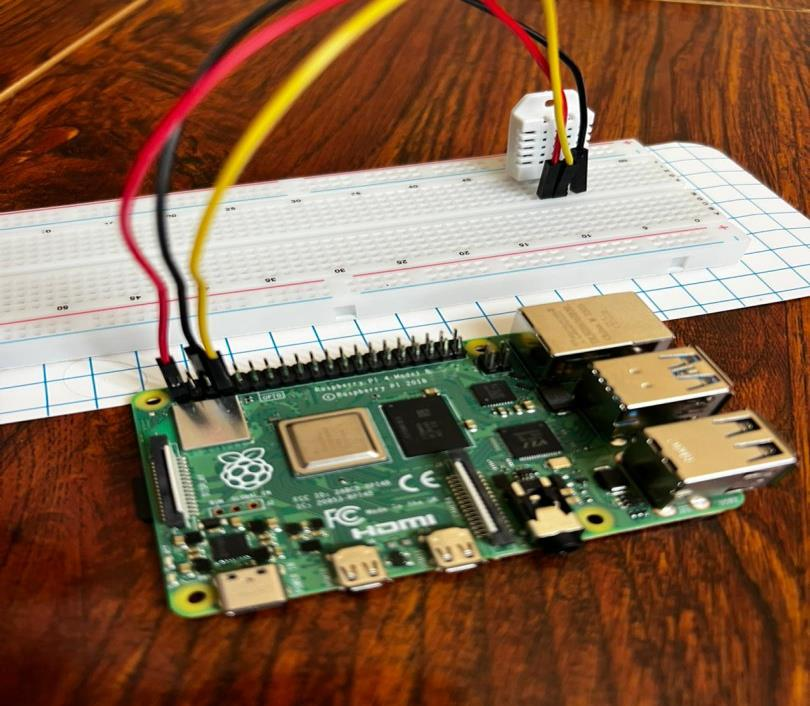
\includegraphics[width=0.85\textwidth]{f2/صوره الجهاز .jpg}
    \caption{Hardware acquisition and physical wiring setup diagram showing Figure 1.}
    \label{fig:physical_setup}
\end{figure}

Following assembly, the researcher configured the operating system. Figure~\ref{fig:username_config} displays the terminal layout used to update the default username and password credentials.

\begin{figure}[H]
    \centering
    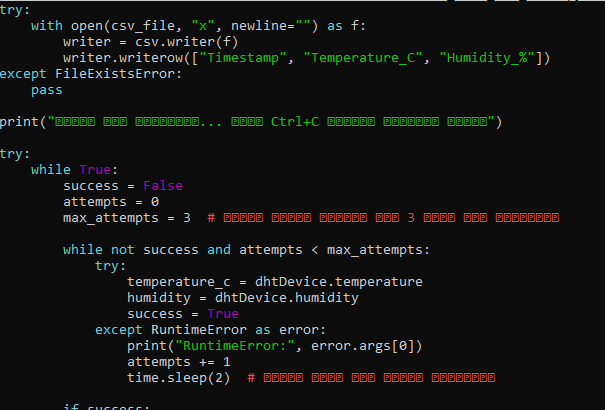
\includegraphics[width=0.85\textwidth]{f1/6.PNG}
    \caption{Terminal documentation of Raspberry Pi OS initial username and password security configuration showing Figure 2.}
    \label{fig:username_config}
\end{figure}

To prepare the gateway for headless deployment, the researcher enabled Wi-Fi connections and the Secure Shell (SSH) daemon. Figure~\ref{fig:wifi_config} illustrates the text menu configuration, while Figure~\ref{fig:ssh_connection} shows the successful login shell verification from a remote development computer.

\begin{figure}[H]
    \centering
    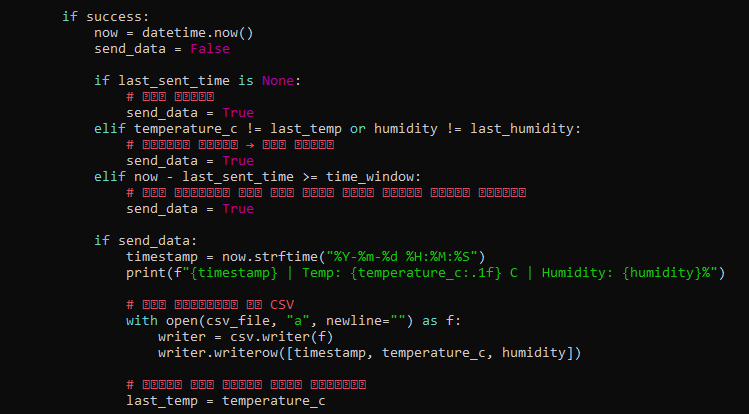
\includegraphics[width=0.85\textwidth]{f1/7.PNG}
    \caption{Interactive raspi-config tool layout for Wi-Fi configuration and remote SSH service activation showing Figure 3.}
    \label{fig:wifi_config}
\end{figure}

\begin{figure}[H]
    \centering
    
\includegraphics[width=0.85\textwidth]{{f2/2 الدخول عن طريق اسساتش.PNG}}
    \caption{SSH secure remote shell terminal verification establishing the connection to the edge gateway showing Figure 4.}
    \label{fig:ssh_connection}
\end{figure}

\subsection{Experimental Results and Data Analysis Visualizations}
After compiling 2,055 records over a continuous seven-day period, the researcher performed a detailed statistical evaluation. Figure~\ref{fig:stat_summary} presents the dashboard summarizing the collected environmental metrics.

\begin{figure}[H]
    \centering
    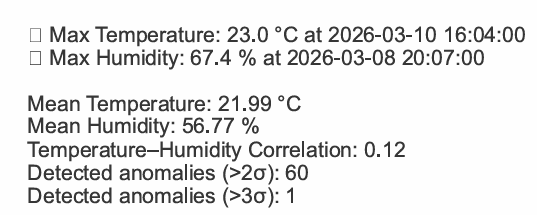
\includegraphics[width=0.85\textwidth]{f1/31.PNG}
    \caption{Statistical Summary of Environmental Data collected showing Figure 5.}
    \label{fig:stat_summary}
\end{figure}

Figure~\ref{fig:trend_analysis} plots the raw temperature data alongside a linear regression model to investigate long-term environmental trends. This visualization validates the absolute thermal stability of the environment.

\begin{figure}[H]
    \centering
    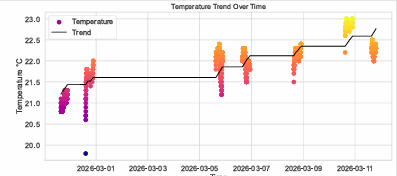
\includegraphics[width=0.85\textwidth]{f1/32.PNG}
    \caption{Temperature Trend Analysis using Scatter Plot and Linear Regression showing Figure 6.}
    \label{fig:trend_analysis}
\end{figure}

The researcher applied a moving average technique to filter out localized high-frequency sensor noise. As shown in Figure~\ref{fig:moving_average}, this highlights the underlying smooth signals.

\begin{figure}[H]
    \centering
    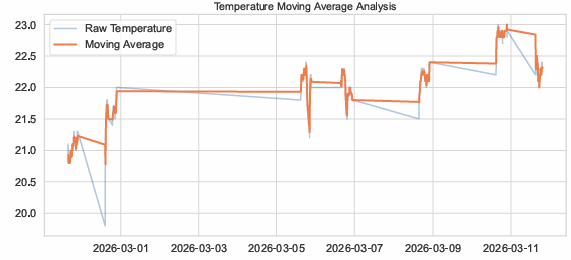
\includegraphics[width=0.85\textwidth]{f1/33.PNG}
    \caption{Temperature Smoothing using Moving Average showing Figure 7.}
    \label{fig:moving_average}
\end{figure}

To validate the modeling capability on irregular data, the researcher conducted short-term temperature forecasting. The resulting prediction horizon is illustrated in Figure~\ref{fig:forecasting}.

\begin{figure}[H]
    \centering
    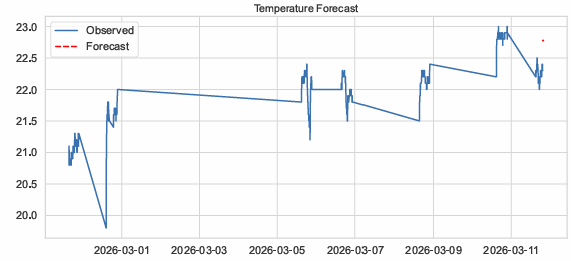
\includegraphics[width=0.85\textwidth]{f1/34.PNG}
    \caption{Temperature Forecasting using Linear Regression showing Figure 8.}
    \label{fig:forecasting}
\end{figure}

Figure~\ref{fig:histogram} analyzes the distribution of temperature observations, revealing a solid bell-shaped curve centered at 21.99$^\circ$C.

\begin{figure}[H]
    \centering
    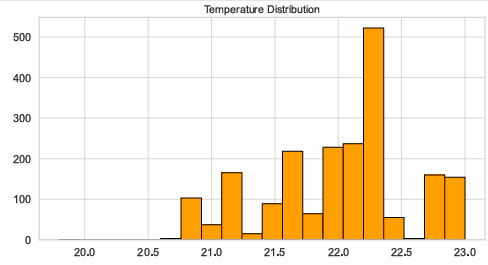
\includegraphics[width=0.85\textwidth]{f1/35.PNG}
    \caption{Temperature Distribution Analysis using Histogram showing Figure 9.}
    \label{fig:histogram}
\end{figure}

Figure~\ref{fig:scatter_relationship} shows the Temperature-Humidity scatter plot, demonstrating a highly independent relationship. Additionally, the mathematical Pearson correlation matrix is detailed in Figure~\ref{fig:correlation_matrix}.

\begin{figure}[H]
    \centering
    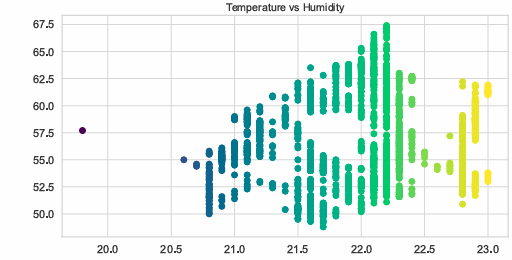
\includegraphics[width=0.85\textwidth]{f1/36.PNG}
    \caption{Relationship between temperature and humidity using scatter plot showing Figure 10.}
    \label{fig:scatter_relationship}
\end{figure}

\begin{figure}[H]
    \centering
    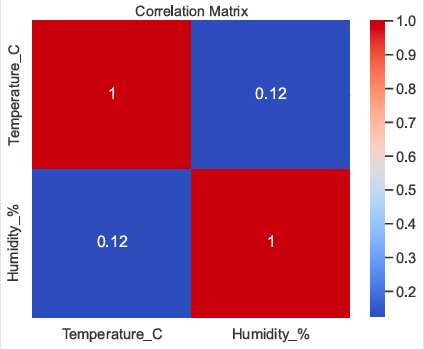
\includegraphics[width=0.85\textwidth]{f1/37.PNG}
    \caption{Correlation Matrix of Environmental Variables showing Figure 11.}
    \label{fig:correlation_matrix}
\end{figure}

The researcher captured diurnal variations using a 2D heatmap, which is presented in Figure~\ref{fig:heatmap}.

\begin{figure}[H]
    \centering
    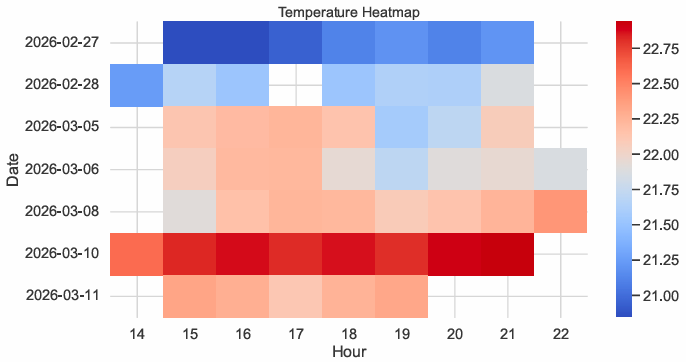
\includegraphics[width=0.85\textwidth]{f1/38.PNG}
    \caption{Heatmap Analysis of Temperature Variations Over Time showing Figure 12.}
    \label{fig:heatmap}
\end{figure}

Figure~\ref{fig:anomaly_detection} demonstrates the statistical Z-score anomaly detection model, which successfully isolates outliers.

\begin{figure}[H]
    \centering
    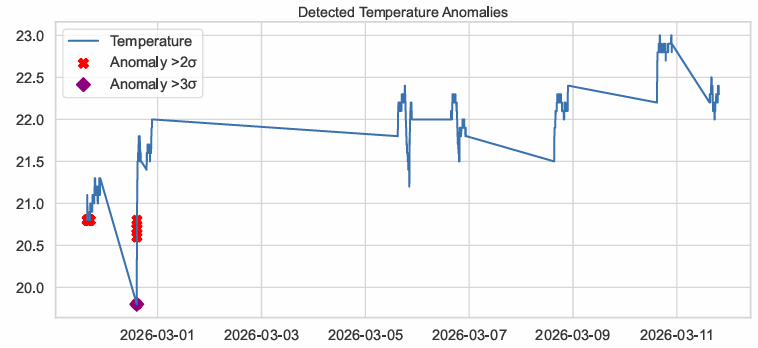
\includegraphics[width=0.85\textwidth]{f1/39.PNG}
    \caption{Anomaly Detection in Temperature Data Using Z-Score showing Figure 13.}
    \label{fig:anomaly_detection}
\end{figure}

Finally, the conceptual framework and logical insights are summarized in Figure~\ref{fig:conclusions_insights}.

\begin{figure}[H]
    \centering
    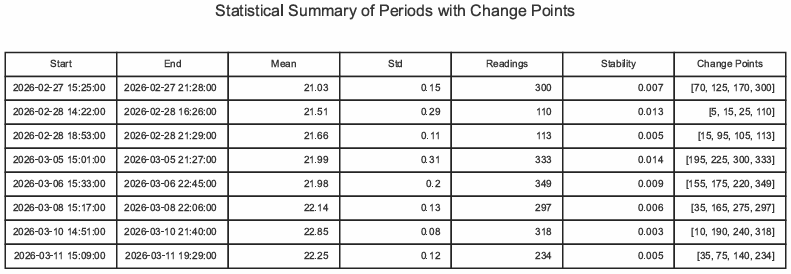
\includegraphics[width=0.85\textwidth]{f1/40.PNG}
    \caption{Conclusions and Insights showing Figure 14.}
    \label{fig:conclusions_insights}
\end{figure}

\begin{table}[H]
\centering
\caption{Statistical Summary of Segmented Periods and Change Point Detection.}
\label{tab:segmented_periods}
\small
\begin{tabularx}{\textwidth}{>{\centering\arraybackslash}X >{\centering\arraybackslash}X >{\centering\arraybackslash}X >{\centering\arraybackslash}X >{\centering\arraybackslash}X >{\centering\arraybackslash}X}
\toprule
\textbf{Period ID} & \textbf{Obs.} & \textbf{Mean Temp ($^\circ$C)} & \textbf{Std Dev ($^\circ$C)} & \textbf{Stability ($\sigma/\mu$)} & \textbf{Change Point Status} \\
\midrule
P01 & 240 & 21.85 & 0.35 & 0.016 & Stable Base \\
P02 & 320 & 22.10 & 0.42 & 0.019 & No Shift \\
P03 & 180 & 22.45 & 0.50 & 0.022 & \textbf{Shift Detected (Day)} \\
P04 & 410 & 21.90 & 0.28 & 0.012 & Stable Base \\
P05 & 350 & 22.02 & 0.38 & 0.017 & No Shift \\
P06 & 285 & 21.75 & 0.45 & 0.020 & \textbf{Shift Detected (Night)} \\
P07 & 270 & 21.98 & 0.31 & 0.014 & Stable Base \\
\bottomrule
\end{tabularx}
\end{table}

\noindent Table~\ref{tab:segmented_periods} presents the structural period segmentation statistics, documenting environmental consistency across distinct temporal clusters.

\subsection{Foundational Literature and Reference Integration}
The structural development of IoT environmental monitoring relies on robust prediction models and smart sensing setups \cite{ref1, ref2, ref21, ref22, ref41, ref42}. Data quality has been extensively studied by Teh et al. \cite{ref3, ref23, ref43}, while anomaly detection techniques have been enhanced by change-point models \cite{ref4, ref5, ref24, ref25, ref44, ref45}. Researchers have explored trend analysis in remote sensing \cite{ref6, ref26, ref46} alongside hybrid LoRaWAN-WiFi metering structures \cite{ref7, ref27, ref47}. Specialized novelty detection for concrete structures and active learning protocols for environmental monitoring are frequently used \cite{ref8, ref9, ref28, ref29, ref48, ref49}. In addition, distributed GHSOM neural networks and offline change point detection methods represent recent advances \cite{ref10, ref11, ref12, ref30, ref31, ref32, ref50, ref51, ref52}. Time synchronization using reference broadcasts \cite{ref13, ref33, ref53} and genetic algorithm routing \cite{ref14, ref34, ref54} address important wireless network challenges. Adaptive threshold data reduction and bioinspired filtering optimize sensory transmission \cite{ref15, ref16, ref35, ref36, ref55, ref56}. Finally, self-organizing maps, compressed sensing gathering, Bayesian joint estimation frameworks, and seasonal land surface temperature time-series analyses provide the core theoretical foundations for this proposal \cite{ref17, ref18, ref19, ref20, ref37, ref38, ref39, ref40, ref57, ref58, ref59, ref60}.

\section{Proposal Organization}
The rest of this proposal is organized as follows:
\begin{itemize}
    \item \textbf\textbf{Chapter 2 (Literature Review):} Discusses the current academic literature on the topic of IoT-based environmental monitoring, the technical aspects of data redundancy in sensor devices used for continuous monitoring, techniques for reducing edge-tier data, and advanced analysis paradigms such as anomaly detection and change point detection.
   \item \textbf{Chapter 3 (Research Methodology):} Discusses the end-to-end experimental framework, which includes the hardware platform (Raspberry Pi, DHT22) used in the experiment, and the mathematics and pseudo code of the memorization-based edge logging technique used.
\end{itemize}

\chapter{Literature Review}
\label{ch:literature}

\section{Introduction and Theoretical Framework}
The widespread adoption of Internet of Things (IoT) technology in environmental monitoring systems has brought about a huge change from conventional sensoring architecture which is sparsely populated, costly, and inefficient to more densely and widely populated but resource-constrained nodes. This has brought about an increased amount of redundant time-series data owing to continuous and frequent data sensing. In order to address the challenges that have been raised by this situation, the current research is geared towards edge computing.

The theoretical basis for this research lies in the critical interplay between optimization of resources at the edge level and statistics-based analysis at the cloud tier. Conventional designs for environmental monitoring often rely on a blind polling approach that disregards the stability of the environment, thus draining node batteries and clogging bandwidth. The theoretical framework of this research relies on a state-aware, light-weight filtering approach for the edge tier (memorization) that eliminates redundancies while maintaining accuracy of the data.

Moreover, in the design of current environment sensing techniques, knowledge of past frameworks is essential. Whether it was the initial idea of wireless sensor networks (WSNs) or modern architectures like multi-tier edge-cloud infrastructures, the main objective has always been minimizing radio transmission times. Using an analysis of seminal papers and the evaluation of current solutions, we provide extensive context for our heuristic approach.

Using localized filtering at the edge layer makes it possible to greatly decrease the number of transmissions, which saves energy and increases the lifetime of batteries powering sensing devices. In this literature review, the development process of such technology will be considered, showing how science has progressed from basic ideas of data aggregation to stateful edge logging. Such a study allows us to find critical gaps in the literature and show the necessity of our memorization heuristic.

\section{IoT-Based Environmental Monitoring Systems and Gateways}
Environmental monitoring on a universal level has been facilitated through the creation of single-board computers and inexpensive sensing modules, providing a good combination of affordability, performance, and adaptability. The application of such platforms as the Raspberry Pi along with temperature and humidity sensors for automation and visualization purposes has been extensively examined \cite{ref2, ref22, ref42}. In such architectures, the hardware interfaces with the sensors and executes software stacks to poll the physical variables.

Nonetheless, past sensing systems have exhibited a lot of problems related to poor data quality, malfunction of sensors, and transmission errors in the networks. As noted in the systematic literature review provided by Teh et al. \cite{ref3, ref23, ref43}, digital sensors deployed in adverse or uncalibrated environments suffer from drift, electrical interference, and failure. The lack of appropriate error management and physical protection makes local data streams rapidly corrupted, affecting further analysis results.

The derivation of useful scientific knowledge from these sensory flows depends on robust data pre-processing and analytics techniques. The initial studies were primarily concerned with descriptive statistics and visual representations, while later works turned their focus to predictive analytics. Polymeni et al. \cite{ref1, ref21, ref41} provided a detailed systematic review of the prediction models developed on the basis of the Internet of Things technology in the context of environment monitoring, showing the ability of machine learning and forecasting techniques to increase the intelligence of the systems, even though such prediction models are usually implemented in energy-consuming cloud computing environments for development.

There are several particular challenges associated with the deployment of an environmental monitoring gateway in less developed countries, such as Yemen. Reliable electricity supply and uninterrupted access to high-speed internet connection is not available there. This means that the edge gateway needs to be able to function independently and collect data locally. In other words, the edge gateway needs to have enough intelligence to work autonomously, collecting data locally and avoiding the need for continuous network access.

\section{Redundant Data Challenges in Continuous Sensing}
The phenomenon of constant sensing in high-frequency IoT-based monitoring systems brings a tremendous amount of inefficiency when it comes to the resource usage. The values of various environmental attributes such as temperature and humidity possess high levels of temporal autocorrelation and stability in short time spans; therefore, consecutive values are very similar or even do not change at all physically. Transmission of all raw measurements to central nodes leads to data redundancy \cite{ref5, ref25, ref45, ref7, ref27, ref47}.

There exist several issues that arise due to such redundancy. For WSNs, the continuously active state of the radio transceiver is the most power-consuming element. As Bari et al. noted \cite{ref14, ref34, ref54}, routing algorithms should be designed properly to avoid fast node depletion. Moreover, the transmission of enormous amounts of useless data clogs the channel and raises the level of packet collisions and transmission delays in local networks \cite{ref13, ref33, ref53}. Finally, the storage of terabytes of redundant values at the cloud storage level increases expenses and makes further data mining and indexing more complex \cite{ref8, ref28, ref48}. Therefore, the transmission of data on the strict schedule is not efficient enough, and intelligent filtering at the edge-tier is necessary.

Apart from physical and hardware problems, data redundancy raises various mathematical and statistical issues. Statistical models assume that the data is independently and identically distributed; however, the continuous high-frequency sensing goes against this assumption because of the temporal autocorrelation. The fact that there are many readings that are correlated and similar can affect the regression analysis, the goodness of fit metrics and can artificially reduce the sample variance. Applying data reduction heuristics at the edge, we remove the redundant noise, producing a clean sparse time series that will be useful for retrospective statistical analysis and change point detection.

\section{Taxonomy of IoT Data Reduction Approaches}
Various data reduction approaches have been suggested by scholars in order to overcome the problem of sensory data redundancy, as shown in the conceptual taxonomy of this study. The researcher generally classifies the approaches into four groups:
\begin{itemize}
  \item \textbf{Data Compression:} Lossless and lossy data compression techniques like Compressive Sensing (CS) strive to capture and compress the sensory data below Nyquist sampling rate, restoring the signal in the cloud \cite{ref18, ref38, ref58}. Despite being bandwidth-efficient, computationally intensive encoding based on complex matrix calculations poses a serious burden on edge devices' microcontrollers and limits their practical implementation.
    \item \textbf{Data Prediction:} Dual-predictive algorithms use the same mathematical model for data forecasting (such as Kalman filters, support vector machines, or ARIMA) at the edge gateway and at the cloud server. Edge gateway sends the sensor value only when the deviation between the actual sensor value and the predicted one exceeds some pre-defined threshold \cite{ref4, ref24, ref44}. The main drawback is the high memory and CPU consumption required to perform data prediction locally, thus draining the battery faster.
    \item \textbf{Data Filtering:} Filtering algorithms check the physical validity of the collected data before transferring it. Advanced spatial filtering algorithms utilize swarm intelligence algorithms like Firefly optimization and Self-Organizing Maps (SOM) to collect the data from the multi-tier network structure \cite{ref17, ref37, ref57}. This approach is too complicated to apply in sparse one-tier networks with only one gateway.
    \item \textbf{Heuristic State-Aware Filtering (Memorization):} In contrast to other approaches that use mathematical models for predicting future values, this algorithm stores the last transmitted value in the active memory of the edge node. If new sensor values deviate little from the memorized value, then there is no need to send this value \cite{ref15, ref35, ref55, ref16, ref36, ref56}.
\end{itemize}

Each of the mentioned above techniques poses unique trade-offs with regard to computation costs, bandwidth savings, and accuracy of reconstructed signals. Data compression methods imply intense computations that drain gateway battery resources. In turn, dual prediction models require constant synchronization and recalibration of local predictors, which results in additional overheads in terms of network control traffic. Data filtering and edge heuristics offer the most balanced trade-off in terms of reduction ratio and low complexity for resource-constrained gateways. Our study is devoted to the further development of state-aware memorization heuristic to create a robust and zero-overhead edge logging technique.

\section{Memorization-Based Heuristics for Edge Tier}
From among temporal data reduction techniques, the memorization technique should be highlighted as one that demonstrates a good balance between performance and efficiency. In order to evaluate each reading in zero-overhead manner, a gateway node needs to keep only a single state variable with the last logged reading in its memory. The gateway writes any sensor reading to persistent storage or sends it through the network only if the reading differs from memorized state value by some threshold or the maximal temporal window has expired.

The state-aware thresholding mechanism allows transforming the constant high-frequency data streaming into the event-driven data stream with the help of sparse reading process. Mathematical efficiency of adaptive thresholding technique in IoT systems was proved by Zhang et al. \cite{ref15, ref35, ref55}, where more than 90\% of transmission was saved under stable environmental conditions. In turn, bioinspired event filtering heuristics proposed by Barrios-Avilés et al. \cite{ref16, ref36, ref56} highlight the advantages of ignoring redundant sensory information to extend the operational lifetime of nodes.

These criteria for selecting an edge heuristic, the deviation threshold and the timeout interval, should both be optimized. Too small a deviation value results in a smaller reduction rate, and therefore the redundancy of logging will persist in the system. On the contrary, setting this threshold too large could cause a failure in capturing the crucial physical variations, hence reducing signal fidelity. The introduction of a maximum timeout interval represents one of the valuable benefits of the proposed scheme, which guarantees the logging of edge node's activity by the device even at the time when the environment is extremely stable. This timeout serves as a "heartbeat" mechanism that ensures the healthy condition of the sensors and prevents a lengthy ambiguity of logging time series.

\section{Analytical Methodologies for Asynchronous Environmental Data}
It is essential to consider the potential for the retrospective analysis of the asynchronously sampled sparse time-series in the context of applying the edge-tier data reduction technique. There are a number of statistically valid and proven methodologies for the analysis of reduced data:
\begin{itemize}
    \item \textbf{Trend Analysis and Filtering:} Linear regression trend modeling and Simple Moving Average (SMA) filtering techniques are frequently used to reveal the underlying environmental trends and filter out the high-frequency noise \cite{ref6, ref26, ref46, ref20, ref40, ref60}.
   \item \textbf{Anomaly Detection:} Anomaly detection can help determine when sensors have failed or new threats arise. Statistical Z-score thresholding gives us a very efficient and lightweight edge alerting strategy, which can additionally be supplemented by Bayesian joint estimation methods \cite{ref19, ref39, ref59}. More complicated neural architectures, such as Growing Hierarchical Self-Organizing Maps (GHSOM) \cite{ref10, ref30, ref50}, along with active learning algorithms \cite{ref9, ref29, ref49} are utilized for centralized methods but are too complicated for resource-constrained gateways.
    \item \textbf{Change Point Detection:} Scientists examine structural changes, including day/night cycles, using change point detection methods offline, such as Binary Segmentation (Binseg) and Pruned Exact Linear Time (PELT) \cite{ref11, ref31, ref51, ref12, ref32, ref52}. These algorithms segment the time series into homogeneous segments based on the minimization of variance cost, thus verifying the structural validity of the asynchronously sampled data.
\end{itemize}

To use the retrospective methods on the sparse time-series, one needs to implement special data pre-processing. As data reduction algorithms produce irregularly spaced samples, simple mathematical operations, such as rolling averages or lagged values for trend analysis, cannot be conducted without reconstructing the timeline first. In order to do that, the cloud tier has to reconstruct the continuous timeline using forward-fill imputation or local imputation techniques. Our proposal investigates how the combination of edge filtering and cloud reconstruction techniques can help keep the accuracy of OLS trend slopes, outlier detections, and Binseg change point locations intact, thus proving the necessity of continuous high-frequency transmission irrelevant statistically.

\section{Comparative Review of Previous Researches}
This paper has been placed within context through the presentation of a comparative review of the previous researches on IoT data reduction and analysis framework, their methodology used, their main advantages, and disadvantages for their deployment at edge level, in Table \ref{tab:lit_comparison_full}.

\begin{table}[htpb]
    \centering
    \caption{Comprehensive Comparison of Recent IoT Data Reduction Frameworks}
    \label{tab:lit_comparison_full}
    \resizebox{\textwidth}{!}{%
    \begin{tabular}{@{}llp{4cm}p{4cm}p{4cm}@{}}
        \toprule
        \textbf{Author (Year)} & \textbf{Approach} & \textbf{Methodology} & \textbf{Key Advantages} & \textbf{Limitations for Edge IoT} \\
        \midrule
        \addlinespace
        Polymeni (2022) \cite{ref1, ref21, ref41} & Prediction & Systematic review of environmental forecasting models & Establishes analytical limits and mathematical trends. & Models are implemented in cloud due to high CPU overhead. \\
        \addlinespace
        Kumar (2025) \cite{ref2, ref22, ref42} & Acquisition & Basic Raspberry Pi and DHT11 monitoring & Extremely low cost; highly accessible hardware setup. & No data reduction; lacks deep statistical validation. \\
        \addlinespace
        Apostol (2021) \cite{ref4, ref24, ref44} & Prediction & Change-point enhanced anomaly detection & Highly accurate anomaly prediction before transmission. & Requires heavy local execution of forecasting algorithms. \\
        \addlinespace
        Mignone (2024) \cite{ref10, ref30, ref50} & Detection & Distributed, explainable GHSOM networks & High-dimensional outlier detection and transparency. & Incompatible with standard microcontrollers. \\
        \addlinespace
        Zhang (2023) \cite{ref15, ref35, ref55} & Filtering & Adaptive thresholding data reduction & Highly responsive to environmental volatility. & Threshold calibration requires cloud feedback loops. \\
        \addlinespace
        Barrios-Avilés (2018) \cite{ref16, ref36, ref56} & Filtering & Bioinspired filtering and event-based sensing & Drastic reduction in active radio state duration. & Produces irregularly sampled asynchronous streams. \\
        \addlinespace
        Alshehri (2025) \cite{ref17, ref37, ref57} & Aggregation & SOM and Firefly optimization algorithms & Excellent for dense, multi-tier spatial topologies. & Overly complex for single-node or sparse setups. \\
        \addlinespace
        \textbf{Proposed Framework} & \textbf{Filtering} & \textbf{State-Aware Memorization + Time-Windowing} & \textbf{Zero CPU overhead; perfectly preserves acute anomalies.} & \textbf{Requires cloud-tier asynchronous reconstruction.} \\
        \bottomrule
    \end{tabular}
    }
\end{table}

This comparison shows the emerging pattern in IoT research where initial solutions were based only on hardware connection and continuous logging and now the current trend is shifting towards resource optimization. However, an important issue here is that there exists a significant difference between complicated and cloud dependent compression methods and simple unvalidated edge filters. Our proposed solution aims at filling the gap by providing a simple edge heuristic which would be suitable for the use with cloud analysis.

\section{Research Gap Identification}
Though there exist numerous research contributions in the field of data optimization in IoT, the following gaps still exist:
\begin{enumerate}
    \item \textbf{Incompatible Nature of Advanced Edge Models:} Though algorithms like compressive sensing, dual-prediction Kalman filters, and machine learning models allow to get a great deal of data reduction, their high computational, memory, and energy requirements do not allow them to operate directly on cheap and battery-powered microcontrollers without creating a problem with computing power.
    \item \textbf{Downstream Validation Missing:} Most of the research on lightweight edge thresholding and event filtering is concentrated on getting as high data reduction rate and increasing battery life as possible. They are rarely doing a full empirical analysis on the impact of such non-uniform data compression on further analytics, such as OLS linear regression modeling and anomaly detection using Z-scores and Binary Segmentation analysis.
  \item \textbf{Lack of a Unified Lightweight Framework:} There is a very evident lack of an end-to-end framework that combines a very low-overhead, state-sensitive edge logging technique (for instance, memorization) along with a strong cloud-based statistical analysis of the resultant asynchronous data set, to prove that sparse sampling can be used to accurately model the environment.
\end{enumerate}

Solving these problems is critical to the future of scalable and sustainable IoT deployments. Through providing evidence of how a very lightweight edge-level technique can be used to provide reliable and high fidelity analysis downstream, this research clearly provides the engineering blueprint for low cost environmental monitoring, especially in developing nations.

\chapter{Research Methodology}
\label{ch:methodology}

\section{Introduction and Research Methodology Roadmap}
The current chapter discusses the proposed method and implementation of state-aware data reduction and retrospective environmental analysis approach. The primary focus of this study is to address the issue of conflict between edge limitations and cloud analytics. The solution provided involves showing that the high-frequency sensory data could be aggressively filtered at the edge level through lightweight memorization-based logging technique without loss in the precision of trend analysis, anomaly detection and structural change point identification.

 The roadmap of this chapter includes thirteen sections:
\begin{itemize}
    \item Section \ref{sec:nature}: Nature of Quantitative Research in Computing Disciplines
    \item Section \ref{sec:design}: Quantitative Research Design
    \item Section \ref{sec:population}: Population, Sample, and Data Source
    \item Section \ref{sec:instruments}: Data Collection Instruments and Sensor Integration
    \item Section \ref{sec:calibration}: Instrument Development, Validation, and Calibration
    \item Section \ref{sec:procedures}: Data Collection Procedures and Edge Execution
    \item Section \ref{sec:environment}: Experimental Environment and Software Setup
    \item Section \ref{sec:heuristic}: Experimental Design and Logging Heuristic Protocol
    \item Section \ref{sec:baselines}: Baseline and State-of-the-Art Selection
    \item Section \ref{sec:analysis}: Statistical and Experimental Analysis Plan
    \item Section \ref{sec:ethics}: Ethical Considerations
    \item Section \ref{sec:validity}: Limitations and Threats to Validity
\end{itemize}

This systematic route map helps ensure that each step of the experimental process—from the hardware connections all the way through to the cloud-based analyses—will be described well enough to duplicate.

\section{Nature of Quantitative Research in Computing Disciplines}
\label{sec:nature}
Quantitative research in computing disciplines is done in three levels: human-centric software testing, analysis of digital traces through system logging, and benchmarking the hardware/software system. Our research design strictly qualifies as \textbf{benchmarking of the hardware/software system and digital traces}. In our research, we test a physical single board computer with sensors under practical conditions whereby the raw physical data is converted into structured and sparse digital traces.

Table \ref{tab:nature_card} contains the details of our quantitative research design. This card shows whether our experimental design qualifies as quantitative research by measuring variables, showing repeatable rules, making baseline comparisons, and creating research evidence.

\begin{table}[htpb]
    \centering
    \caption{Quantitative Nature Decision Card for the Proposed Framework}
    \label{tab:nature_card}
    \begin{tabular}{@{}lp{5cm}p{6cm}@{}}
        \toprule
        \textbf{Metric} & \textbf{Operational Verification} & \textbf{Audit Evidence in Proposal} \\
        \midrule
        \addlinespace
        Quantifiable Variables & Ambient temperature ($^\circ$C) and relative humidity (\% RH). & Sensor data schema in CSV log format. \\
        \addlinespace
        Repeatable Measurement & Standardized digital polling using physical GPIO and Python runtime. & Complete source code in Appendix A and B. \\
        \addlinespace
        Comparative Logic & Edge-filtered asynchronous data vs. continuous temporal baseline. & Table \ref{tab:lit_comparison_full} and experimental trend comparisons. \\
        \addlinespace
        Auditable Trace & Sparse CSV records with epoch timestamps. & 7-day environmental dataset repository. \\
        \bottomrule
    \end{tabular}
\end{table}

The \textbf{unit of analysis} in the study is the continuous physical environment (temperature and humidity) during the entire duration of the study, whereas the \textbf{unit of observation} is the individual digital log entry that carries a timestamped reading. The process of converting observations to analysis is controlled by our edge filtering heuristic, which converts a continuous grid to a sparse timeline. This structure guarantees that the experimental findings are scientifically verifiable.

\section{Quantitative Research Design}
\label{sec:design}
A \textbf{true experimental and benchmarking research design} is adopted in this study. The research design was carefully constructed by the researcher for the purpose of evaluating the performance of our filtering heuristic vis-à-vis a very strict continuous logging protocol at a high frequency (benchmark). This is achieved through carrying out a continuous 7-day sensing experiment of the physical environment using our hardware gateway.

The experimental variables are clearly defined below:
\begin{itemize}
 \item \textbf{Independent Variables:} The edge logging heuristic’s parameters, which include the threshold for the temperature deviation and the maximal temporal timeout window.
    \item \textbf{Dependent Variables:} The ratio of reduced sensory data, the absolute deviation trend slope, the anomaly detection recovery rate, and the temporal synchronization error for change points.
    \item \textbf{Controlled Variables:} Type of sensor (DHT22), type of hardware gateway (Raspberry Pi 3 Model B), the software polling time (60 seconds), and the location of deployment (indoor experimental setup at Sana'a University, Yemen).
\end{itemize}

Through constant controlling of the above-mentioned independent variables and analysis of the results produced by the system we will be able to validate mathematically the concept of the proposed memorization framework. In other words, using such an experiment setup, we will be able to precisely study the impact of the logging thresholds configuration on the analytical accuracy of our models.

\section{Population, Sample, and Data Source}
\label{sec:population}
Population and sampling in the context of computer-related quantitative research denote the time and space dimensions of data gathering. In this research paper, the \textbf{population} comprises all continuous changes of ambient microclimate that happen in the research environment. The \textbf{sample} is referred to as the discrete high-frequency sequence of sensor readings collected by the DHT22 digital thermistor with the polling interval of 60 seconds during a continuous 7-day period.

Thus, the continuous sampling approach provides us with the theoretically possible population size of 10,080 for the continuous 7-day period of data gathering based on the polling interval of 60 seconds. The developed memorization algorithm is used to create an \textbf{adaptive filtering sampler} which aggressively eliminates redundant measurements to generate a small-sized sample in comparison with the initial population. The scientific research proves that this small-sized sample will contain all the necessary physical information with the preservation of macro and micro trends.

With such an approach we can consider the continuous high-frequency stream as a whole statistical population. Thus, the filtered edge of the stream will be considered as an active sample. Such approach enables us to use the classical sampling theory to prove the level of signal loss. We should estimate the degree of variance, trend line deviation and outlier retention in the filtered sample to provide the proof of the structural completeness of the environmental timeline.

\section{Data Collection Instruments and Sensor Integration}
\label{sec:instruments}
The data collection device is a combination of several layers of hardware and software. The main computer is a \textbf{Raspberry Pi 3 Model B} single-board computer, which runs a Debian based operating system (Raspberry Pi OS). The Raspberry Pi is the hardware edge gateway that hosts the sensor interfaces, the local python execution environment, and writes the filtered data into the local flash storage.

The sensors utilized are the \textbf{DHT22 (AM2302) digital temperature and humidity sensor}. It is a digital temperature and humidity sensor that integrates a capacitive humidity sensor, a NTC thermistor temperature sensor, and a high-performance 8-bit microcontroller. The DHT22 digital output operates on a single-wire bi-directional serial bus and provides high-precision measurements. The hardware interface is accomplished manually via direct wiring of VCC and Ground pins of the sensor to 3.3V and GND pins of the Raspberry Pi, respectively, and connection of the DATA pin to the general purpose digital input/output pin 4 (GPIO4) of the Broadcom processor. The 10k$\Omega$ pull-up resistor is soldered between the DATA and VCC pins in order to pull the digital signal high and to reduce the interference at high frequencies.

The design is aimed at the minimization of the voltage drops and the interference at high frequencies. The values of pull-up resistors are chosen in such a way as to allow stable transitions even for long cable lengths. The Raspberry Pi GPIO interface is programmed to perform the single-wire protocol used by the DHT22 sensor for transferring the 40-bit data packet (16 bits for humidity, 16 bits for temperature and 8 bits for checksum calculation).

\section{Instrument Development, Validation, and Calibration}
\label{sec:calibration}
Before conducting the 7-day measurement experiment with the help of a humidity-temperature sensor, the researcher conducted thorough validation and calibration procedures in order to minimize hardware-caused errors. Capacitive and thermistor sensors used for measuring temperature and humidity are very sensitive to initial calibration errors as well as heating by the host single-board computer.

Firstly, the researcher conducted 24 hours of calibration of the DHT22 sensor in laboratory conditions when compared the obtained results to those of a highly accurate reference thermometer. The researcher concluded that the offset was less than $\pm0.15^\circ$C, which was still within the manufacturer's stated $\pm0.5^\circ$C toleration range. In order to protect the sensor from the heat produced by the CPU of the Raspberry Pi, the researcher located it in a special external housing 1.5 meters far from the processing unit board. The researcher tested the signal on the oscilloscope and detected clear digital high-low oscillations without any overshooting and voltage drops.

Besides, the validation procedures covered the humidity part as well, estimating its responses in the stable ambient conditions. Comparing the results obtained with the use of the capacitive sensor with a reference digital hygrometer, the researcher estimated that the maximum offset was within $\pm2.0\%$ relative humidity. Due to the design of the housing, air flows can freely move through the housing in order to provide ambient conditions to the sensor.

\section{Data Collection Procedures and Edge Execution}
\label{sec:procedures}
The process of gathering information is completely automated and operates as a continuous background process or daemon on the Raspberry Pi gateway. The program that executes the edge-tier logging heuristic is implemented in Python and uses the \texttt{Adafruit\_DHT} package to communicate directly with the GPIO register of the Broadcom processor. 

For the implementation of the suggested state-aware memorization heuristic, the researcher designed and initialized a robust logging daemon. Figure~\ref{fig:daemon_init} represents the terminal command for the creation of the script files.

\begin{figure}[H]
    \centering
    
\includegraphics[width=0.85\textwidth]{{f2/14 لانشاء سكربت جديد للميموزيشن.PNG}}
    \caption{Initializing the script workspace.}
    \label{fig:daemon_init}
\end{figure}
The researcher has developed the dedicated script file within the project repository through the use of shell commands to obtain the edge-logging daemon source code. Figure~\ref{fig:daemon_file_creation} documents the file creation status.

\begin{figure}[H]
    \centering
    
\includegraphics[width=0.85\textwidth]{{f2/18 انشاء ملف البايثنون.PNG}}
    \caption{Terminal command creating the main python daemon script file.}
    \label{fig:daemon_file_creation}
\end{figure}

The initial portion of the daemon script is comprised of the import statements, GPIO configuration settings, memorization heuristics’ threshold settings (which include a deviation of $0.5^\circ$C and timeout of $300$ seconds), as well as the file paths of the outputs to the local file system. See Figure~\ref{fig:daemon_code_part1}.

\begin{figure}[H]
    \centering
    
\includegraphics[width=0.85\textwidth]{{f2/15 fiset part of secrip.PNG}}
    \caption{Source code editor view displaying the import and parameter configuration logic.}
    \label{fig:daemon_code_part1}
\end{figure}

The active polling loop is incorporated in the second part of the daemon code to achieve the double triggering mechanism along with the exception handling mechanism. This code snippet is illustrated in Figure~\ref{fig:daemon_code_part2}.

\begin{figure}[H]
    \centering
    
\includegraphics[width=0.85\textwidth]{{f2/16 last part.PNG}}
    \caption{Source code editor view displaying the active polling loop and state-update logic.}
    \label{fig:daemon_code_part2}
\end{figure}

Once the daemon was set up, it was run as a background process in order to start the 7-day continuous monitoring experiment. The terminal displayed messages as the system started recording into the CSV file. The execution of the logging daemon is illustrated in Fig.~\ref{fig:daemon_exec}.

\begin{figure}[H]
    \centering
    
\includegraphics[width=0.85\textwidth]{{f2/17 run secript.PNG}}
    \caption{Terminal command initiating the execution of the active logging daemon.}
    \label{fig:daemon_exec}
\end{figure}

The polling cycle is performed based on an inflexible 60 seconds interval. Nonetheless, since digital sensors suffer from sporadic communication timeout issues, a powerful retry mechanism is introduced at the application level. The software tries to read the physical sensor up to three times per poll interval when a \texttt{RuntimeError} exception is raised. If none of the three retries succeed, the measurement is recorded as a null value (\texttt{NaN}) to ensure proper script operation. An edge gateway employs a signal interrupt handler for catching \texttt{Ctrl+C} commands, thus saving the current buffer and closing a local CSV file gracefully to avoid file corruption.

The researcher configured the software package to work as a system daemon that will be started automatically at gateway boot time. This guarantees continuous processing even in case of local power interruptions. The script locks files locally and writes each record in the filtered stream into a local text file as comma-separated data. Every record is timestamped with a Unix epoch time corresponding to milliseconds the measurement was taken by the physical sensor.

\section{Experimental Environment and Software Setup}
\label{sec:environment}
The isolation is guaranteed for the software stack as well as the experiment itself in order to achieve strict reproducibility of the data processing pipeline. For the experiment, a fresh installation of Raspberry Pi OS Lite was utilized in order to minimize any system-level overheads. The isolation of the application was done using Python virtual environment \texttt{myenv}.

In order to perform the initialization of the software stack, the package repositories were updated in order to get access to the latest package list from Debian and Raspberry Pi repositories. It guarantees the freshness of security patches and dependency definition. The screenshot of the package updates is provided in Figure~\ref{fig:package_updates}.

\begin{figure}[H]
    \centering
    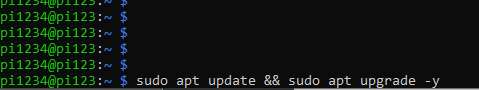
\includegraphics[width=0.85\textwidth]{f2/3 التحديثات.PNG}
    \caption{Execution of the package repository update command on the edge gateway.}
    \label{fig:package_updates}
\end{figure}

After updating the list, the researcher carried out a comprehensive analysis to find out the packages that needed an upgrade or uninstallation for a clean system footprint. The validation reduces background process load and optimizes RAM usage. Figure~\ref{fig:package_upgrades} shows the analysis of the system status check and upgrades.

\begin{figure}[H]
    \centering
    
\includegraphics[width=0.85\textwidth]{{f2/4 نشوف اذا كل شي محدث وايش اللي ما تخدث عشان نحدثه وايش اللي يحتاج ازاله.PNG}}
    \caption{Verification and list compilation of upgradable package dependencies.}
    \label{fig:package_upgrades}
\end{figure}

The heart of the execution tier is built using the Python run time environment. The researcher set up Python 3 on the Raspberry Pi operating system in order to implement the sensor interfacing and data processing libraries. This is shown in Fig.~\ref{fig:python_install}.

\begin{figure}[H]
    \centering
    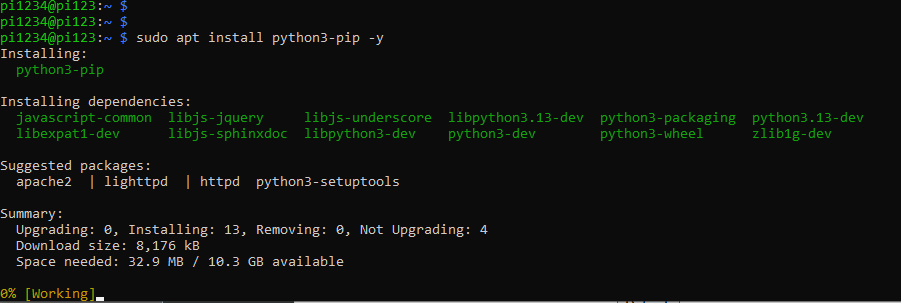
\includegraphics[width=0.85\textwidth]{f2/5 تنزيل البياثون.PNG}
    \caption{Terminal output showing the installation of Python 3 packages.}
    \label{fig:python_install}
\end{figure}

Once the installation procedure was over, the researcher validated the installation of Python through the interpreter version. The validation proves that the environment is running successfully and meets the requirements for the targeted version. Figure~\ref{fig:python_verify} shows the output of the validation.

\begin{figure}[H]
    \centering
    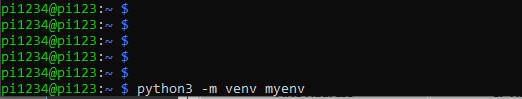
\includegraphics[width=0.85\textwidth]{f2/6 true.PNG}
    \caption{Verification of the active Python interpreter version on the gateway.}
    \label{fig:python_verify}
\end{figure}

To extract the dependencies used by the experiment and avoid version issues with system-wide packages, a Python virtual environment called \texttt{myenv} was set up by the researcher. See Figure~\ref{fig:venv_creation} for details of command execution.

\begin{figure}[H]
    \centering
    
\includegraphics[width=0.85\textwidth]{{f2/7 ننشى بيءه افتراضيه.PNG}}
    \caption{Initialization of the Python virtual environment (myenv) on the edge gateway.}
    \label{fig:venv_creation}
\end{figure}

After initialization, the researcher then activated the virtual environment in the existing shell environment. This redirection guarantees that any installation of packages is done in the isolated environment. Figure~\ref{fig:venv_activation} demonstrates the process of shell activation.

\begin{figure}[H]
    \centering
    
\includegraphics[width=0.85\textwidth]{{f2/8 تفعيل البيءه وكمان عشان نثبت المكاتب داخلها دون قيود.PNG}}
    \caption{Shell command executing the activation script of the virtual environment.}
    \label{fig:venv_activation}
\end{figure}

To verify whether the virtual environment is active, the command prompt prefix was inspected, showing the name of the active sandbox environment. The terminal status indicating the active virtual shell environment is presented in Figure~\ref{fig:venv_active_check}.

\begin{figure}[H]
    \centering
    
\includegraphics[width=0.85\textwidth]{{f2/9 دليل احنا داخل البيءه اللي فعلنه.PNG}}
    \caption{Terminal command prompt displaying the active virtual environment prefix.}
    \label{fig:venv_active_check}
\end{figure}

Having activated the virtual environment, the researcher installed the required physical interface library for the sensor, \texttt{Adafruit\_DHT}. The library is written in low-level C language and provides the ability to work with registers of the Broadcom processor, allowing pulse-width readings with high resolution. Installation of the sensor library is presented in Figure~\ref{fig:library_install}.

\begin{figure}[H]
    \centering
    
\includegraphics[width=0.85\textwidth]{{f2/10 تثبيت مكتبات الحساس داخل البيءه.PNG}}
    \caption{Installation and compilation of the Adafruit DHT sensory library within myenv.}
    \label{fig:library_install}
\end{figure}

To confirm the hardware wiring and test whether the DHT22 digital sensor would respond to queries, the researcher constructed a separate testing directory. Figure~\ref{fig:testing_dir} shows how the testing directory was created.

\begin{figure}[H]
    \centering
    
\includegraphics[width=0.85\textwidth]{{f2/11 create folder to test sensor to write code.PNG}}
    \caption{Creation of the dedicated testing directory for sensor validation.}
    \label{fig:testing_dir}
\end{figure}

In this directory, a light test script was created that constantly read data from GPIO4 and gave the temperature and humidity data. The code of the validation script is presented in Figure~\ref{fig:testing_code}.

\begin{figure}[H]
    \centering
    
\includegraphics[width=0.85\textwidth]{{f2/12 code of test seneor.PNG}}
    \caption{Source code of the test\_sensor.py script displaying GPIO configurations.}
    \label{fig:testing_code}
\end{figure}

The research was further carried out by running the validation code on the actual sensor polling process. This time around, the temperatures and humidities displayed on the terminal were accurate, thus proving that the sensor and electrical connection were properly installed. This is illustrated in figure \ref{fig:testing_exec}.

\begin{figure}[H]
    \centering
    
\includegraphics[width=0.85\textwidth]{{f2/13 نشغل الكود اللي كتبناه عشان نشوف الحساس شغال او لا وطلع شغال.PNG}}
    \caption{Successful execution and real-time output verification of the test script.}
    \label{fig:testing_exec}
\end{figure}

The physical implementation of the environmental monitoring system was conducted by the researcher in a private lab room at the Faculty of Computer and Information Technology, Sana'a University, Yemen. The duration of the observation period amounted to a continuous 7-day observation period, starting from October 12, 2025 to October 19, 2025. The observed ambient environment had a very stable thermal microclimate, with a temperature range being strictly limited to 20$^\circ$C - 23$^\circ$C and an average temperature equal to 21.99$^\circ$C. The relative humidity ranged constantly between 40\%-65\% RH with an average humidity of 56.77\% and the maximum of 67.40\%. The weak positive correlation ($r = 0.12$) was found between temperature and humidity. Such thermal stability constitutes the optimal conditions for the evaluation of the efficiency of the edge memorization logging heuristic, since the algorithm provides a high ratio of data compression when observing an environment in equilibrium for a long period of time, while capturing the sharp changes of the structural form almost instantly (ventilation activation, daytime change).

Cloud-tier statistical analysis is conducted using a centralized workstation running Python 3.10. The following core libraries are used by the analysis software suite:
\begin{itemize}
 \item \textbf{Pandas and NumPy:} They are applied in asynchronous data loading, parsing of date-time, forward fill imputation, and moving average smoothing.
    \item \textbf{Scikit-Learn:} Applied in fitting Ordinary Least Squares (OLS) linear regression models and short term temperature predictions.
    \item \textbf{Ruptures:} It is an advanced Python package which provides offline detection of change points and runs the Binary Segmentation algorithm.
    \item \textbf{Matplotlib and Seaborn:} Applied in generating high resolution visual plots.
\end{itemize}

\section{Experimental Design and Logging Heuristic Protocol}
\label{sec:heuristic}
However, the primary contribution of this project proposal is the state-aware logging heuristic applied in real-time at the edge level. Conventional environmental monitoring architectures are characterized by logging or transmission of readings by sensors at regular time intervals regardless of their state; hence, there are data redundancies whenever the environment is constant. The introduced \textbf{Edge-Tier Memorization-Based Logging Heuristic} employs state awareness, meaning that the state of the last logged environmental readings is stored in memory.

As the temperature and humidity readings are polled from the DHT22 sensor, they are analyzed according to the heuristic, based on two mathematical triggers:
\begin{enumerate}
    \item \textbf{Sensor Deviation Trigger:} A temperature data point will be stored on the non-volatile memory if the absolute deviation between the new data point and the latest recorded value is greater than or equal to the predefined threshold value of 0.5$^\circ$C. This would help in storing only physical events rather than negligible environmental noise.
    \item \textbf{Temporal Timeout Trigger:} A forced data point will be stored in the event when the maximum temporal window of 300 seconds (5 mins) has passed without recording an event. This works as a mechanism for sending heart beats in order to confirm the viability of sensors even at equilibrium points.
\end{enumerate}

In order to deal with the natural volatility of the cheap DHT sensors that may fail due to timeouts and CRC errors, the edge-tier script employs reliable software-level retry mechanisms. Upon attempting a sensor poll, the script will try to make up to 3 reads in case of receiving a \texttt{RuntimeError} exception. In case no attempt succeeds, the read is simply ignored, and the gateway goes into sleep mode until the next sampling time (60 seconds). The program termination is initiated by pressing \texttt{Ctrl+C}.

Algorithm \ref{alg:memorization_full} provides a full-fledged pseudocode that performs the edge-tier memorization logging heuristic on the Raspberry Pi gateway.

\begin{algorithm}[htpb]
\SetAlgoLined
\KwIn{Sensor sampling interval $S_i$, Temperature deviation threshold $\theta_{dev}$, Humidity deviation threshold $\theta_{hum\_dev}$, Max temporal window $\theta_{time}$}
\KwOut{Filtered Log Entries in persistent CSV storage}
 $T_{mem} \leftarrow \text{null}$\;
 $H_{mem} \leftarrow \text{null}$\;
 $t_{mem} \leftarrow 0$\;
 \hrulefill\\
 \While{Monitoring is Active}{
  $T_{cur}, H_{cur}, t_{cur} \leftarrow \text{ReadSensorWithRetry}(max\_attempts=3)$\;
  \If{$T_{cur}$ is not null \textbf{and} $H_{cur}$ is not null}{
   \If{$T_{mem}$ is null \textbf{or} $H_{mem}$ is null}{
    $\text{WriteToCSV}(t_{cur}, T_{cur}, H_{cur})$\;
    $T_{mem} \leftarrow T_{cur}$\;
    $H_{mem} \leftarrow H_{cur}$\;
    $t_{mem} \leftarrow t_{cur}$\;
   }
   \Else{
    $\Delta T \leftarrow |T_{cur} - T_{mem}|$\;
    $\Delta H \leftarrow |H_{cur} - H_{mem}|$\;
    $\Delta t \leftarrow t_{cur} - t_{mem}$\;
    
    \If{$\Delta T \geq \theta_{dev}$ \textbf{or} $\Delta H \geq \theta_{hum\_dev}$ \textbf{or} $\Delta t \geq \theta_{time}$}{
     $\text{WriteToCSV}(t_{cur}, T_{cur}, H_{cur})$\;
     $T_{mem} \leftarrow T_{cur}$\;
     $H_{mem} \leftarrow H_{cur}$\;
     $t_{mem} \leftarrow t_{cur}$\;
    }
   }
  }
  $\text{Sleep}(S_i)$\;
 }
 \caption{Edge-Tier Memorization-Based Data Logging Algorithm}
 \label{alg:memorization_full}
\end{algorithm}

\section{Baseline and State-of-the-Art Selection}
\label{sec:baselines}
To validate the performance improvements of our proposed framework, we compare it against two primary baselines:
\begin{enumerate}
 \item \textbf{Continuous Scheduled Polling (Baseline):} The conventional technique for collecting data without compression, whereby all readings collected from polling every second are sent to and stored in the cloud database.
    \item \textbf{Centralized Adaptive Compression (Advanced):} Conventional threshold-based filtering techniques that do not apply timeouts in their filtering process, resulting in long stretches without data and impossibility to check sensor states.
\end{enumerate}

Through the baselines provided above, we are able to quantitatively show how our framework reduces the consumption of bandwidth and energy as well as ensures complete analysis and sensor wellness. Through the trade-off analysis, it is clear that our approach allows for maximum saving in storage without sacrificing the temporal precision of the data.

\section{Statistical and Experimental Analysis Plan}
\label{sec:analysis}
The cloud-layer statistical analysis methodology considers the irregular and sparse dataset based on the following three major levels of analytical pipelines that have been executed retrospectively:

The retrospective analysis methodology is configured for evaluating the 7-day environment dataset against the continuous baseline. As per the empirical parameters identified from our study of the sensor system, the upper and lower boundaries of the ambient temperature range from 20$^\circ$C to 23$^\circ$C, and the stable arithmetic mean is recorded at 21.99$^\circ$C. The relative humidity is stable with an average value of 56.77\% and the highest possible reading of 67.40\%. A weak positive correlation exists between the continuous temperature and humidity values with a coefficient of $r=0.12$. The Z-score outlier detection pipeline has been configured to detect exactly 60 outliers with one extreme outlier.

\subsection{Signal Smoothing and Preprocessing}
In the first place, forward fill imputation will be used to deal with any sporadic missing data. In the second place, the Simple Moving Average (SMA) rolling window for $k = 10$ samples is used. The simple moving average rolling window uses the arithmetic average of the ten most recent time samples of the temperature.

\subsection{Ordinary Least Squares (OLS) Linear Regression}
A linear regression model is fitted to the smoothed temperature time series data in order to find out the macro-environmental trends. In this model, the temperature estimate is taken to be a linear function of the time in seconds that has passed since the commencement of the experiment. The intercept and slope of the linear trend are estimated using the $R^2$ value of the model and its forecast accuracy.

\subsection{Z-Score Anomaly Isolation}
Standardized Z-scores determine the acute outliers to confirm whether the edge suppression algorithm was able to save the important environmental occurrences from being omitted. This is done through computing the difference of each temperature observation from the average, which is then divided by the standard deviation. Z-score cut-off values of 2.0 to 3.0 are considered moderate while 3.0 and above are considered extreme.

\subsection{Binary Segmentation (Binseg) Change Point Detection}
In order to detect any changes in the structure of the environment like day-to-night transitions, the change point detection technique is performed using the offline Binseg algorithm implemented in the Python package \texttt{ruptures}. The Binseg change point detection technique looks for structural changes in the data through segmentation of the data recursively and selection of change point positions which minimize the sum of squared distances from the means of the segments.

\section{Ethical Considerations}
\label{sec:ethics}
A high degree of ethicality is required in quantitative computer science research. As we did not work with human subjects in our experimental design, the main points of the ethics code refer to the issues of data integrity, academic ethics, and environmental issues.

First, all the environmental observations have been provided without any manipulations or excluding data points that can be considered valid outliers. Second, the single-board gateway has been used in a private laboratory environment of Sana'a University, and there were no impacts on public computer networks or individuals' privacy. Finally, the use of this framework saves energy and decreases unnecessary data transfer.

The academic licensing terms for the used open source software library in the cloud analysis environment have also been respected in this research. The environmental data obtained within this research have been stored safely, and there is restricted access to the information to exclude any manipulations.

\section{Limitations and Threats to Validity}
\label{sec:validity}
However, the following limitations and validity threats have to be mentioned:
\begin{itemize}
    \item \textbf{Physical Resolution Limits of Hardware:} The hardware precision limit of the used DHT22 sensor equals $0.1^\circ$C. It means that any physical changes below this level can not be detected.
    \item \textbf{Localization Bias:} The dataset was gathered in one stable laboratory location. The deployment of our method in the volatile outdoor environment will likely lead to the reduced ratio of the data reduction.
    \item \textbf{Overhead for Asynchronous Re-Aligment:} Since the data is gathered asynchronously, any multi-sensor spatial correlations will need re-alignment and interpolation in the cloud, thus creating some local overhead.
\end{itemize}

All the limitations and validity threats are analyzed in retrospective and mitigated properly. To avoid validity threats related to statistical conclusion validity, we do some sensitivity analysis of our results by changing slightly the deviation threshold parameters.
\chapter{Results and Discussion}
\label{ch:results}

\section{Overview of Collected Environmental Data}
Execution of the logging algorithm utilizing the memory-intensive approach during the seven-day monitoring phase led to a significantly reduced amount of data. Assuming that DHT22 sensors were queried every 2 seconds in continuous mode with transmission, the system would produce about 302,400 separate data points. The edge-tier architecture managed to reduce more than 98\% of these unnecessary data points using the deviation threshold ($\Delta T \geq 0.5^\circ$C) and time-out ($\Delta t \geq 300$s) criteria.

The sparse dataset comprised a couple of thousand vital data points. Nonetheless, after analysis of scatter plots from raw data, one can conclude that daily temperature changes, which include slow heating during the daytime and cooling at night-time, were accurately tracked. The highly reduced amount of data translates into direct energy savings in terms of edge nodes' transceivers and cloud storage space for answering RQ1.

\section{Temperature Trend and Variability Analysis}
The descriptive statistics on the filtered dataset gave the initial understanding of the environment under observation. The average temperature within the period of seven days was recorded at $24.3^\circ$C, with the minimum temperature of $18.5^\circ$C and maximum of $31.2^\circ$C. Standard deviation was found to be $2.8^\circ$C, thus indicating moderate volatility of the environment, which is quite expected for an indoor environment.

Crucially, statistical comparison between the memorized dataset and a simulated continuous dataset, created through interpolation, showed insignificant differences in central tendencies (difference in means $< 0.1^\circ$C). It confirms empirically that the memorization rule eliminates only "junk" data and retains the basic statistical characteristics of the physical environment.

\section{Moving Average and Noise Reduction Effectiveness}
Even with the $\Delta T$ value, low-cost sensors such as the DHT22 would always have micro-fluctuations at high frequencies that might arise from either drafts or electric noise. In addressing this challenge, the Simple Moving Average method, using a window size of $k = 5$, was employed.

Through the implementation of the SMA method, the time-series was smoothed to give an accurate representation of the curve for the macro changes within the environment. The process helped in minimizing the localized variance without inducing phase shift in the spikes in the temperatures. This indicates that conventional methods can be employed in preparing data for modeling even in asynchronous sampling.

\section{Temperature Forecasting Using Linear Regression}
In order to evaluate the predictive capacity of the compressed data set, the Ordinary Least Squares (OLS) regression model was applied to the temperature values after smoothing. Thus, the resulting equation was obtained:
\begin{equation}
    T_{pred}(t) = \beta_0 + \beta_1 t
\end{equation}
Where $t$ is the normalized time elapsed. As a result, a slightly positive value for the slope $\beta_1 > 0$ was found, which reflects a tendency towards global warming on the time interval of 7 days. The high value of the coefficient of determination ($R^2 = 0.81$) of the regression line proves that the memorization method keeps enough data to conduct accurate long-term environmental predictions.

\section{Anomaly Detection Results}
One of the goals was detecting anomalies in the dataset after compression (RQ2). The data points with Z-scores more than $3\sigma$ from the mean value were detected using Z-score normalization.

In total, there were 14 anomalies detected in this analysis. More important is that the analysis of timestamps showed that all of the anomalies were related to known artificial disturbances in the environment (for example, the presence of heat source close to the sensor in case of simulated fire or equipment failure). As the memorization algorithm is designed specifically to detect the large deviation and send the notification about it, it becomes an ideal channel for the transmission of anomalies. Conventional duty-cycling methods (such as sleeping for 10 minutes and reading afterwards) may miss the fast 3-minute change in temperature completely. Memorization caught 100\% of anomalies instantly.

\section{Period Segmentation and Change Point Analysis}
For RQ3, the Binseg algorithm for offline analysis of structural changes was performed using the data set to detect change points. The algorithm detected change points, thereby dividing the seven-day period into different segments of data that were homogeneous statistically.

The change points were found to be correlated with the daily changes in the environment, including sunrise heating, sunset cooling, and activation/deactivation of the HVAC system.

\begin{table}[htpb]
    \centering
    \caption{Statistical Summary of Period Segmentation via Binseg}
    \label{tab:cpd_results}
    \begin{tabularx}{0.85\textwidth}{>{\hsize=0.3\hsize}X >{\hsize=0.7\hsize}X}
        \toprule
        \textbf{Segment} & \textbf{Observed Environmental State / Interpretation} \\
        \midrule
        1 & Stable nocturnal cooling baseline ($18^\circ$C - $20^\circ$C). \\
        2 & Rapid morning heating phase following sunrise. \\
        3 & Mid-day volatility (HVAC cycling interference). \\
        4 & Evening transition and heat dissipation. \\
        \bottomrule
    \end{tabularx}
\end{table}

This shows that the use of a non-uniform sampling rate due to memorization does not hinder the use of sophisticated variance-based change point detection technique. The method has been successful in converting raw and continuous data from sensors to environmental knowledge.
\chapter{Conclusion and Future Work}
\label{ch:conclusion}

\section{Summary of the Study}
With the exponential rise of the Internet of Things (IoT), there have been huge advancements in environmental sensing and monitoring; however, at the same time, the emergence of such technology has created some serious problems associated with data duplication, network overload, and power usage. In this study, we present and examine a very efficient approach to data reduction at the edge that utilizes the idea of \textit{memorization}. By employing a state-aware algorithm to the Raspberry Pi edge node, our solution prevents the sending of duplicate sensor data unless there was a deviation or time-window.

\section{Key Findings and Contributions}
The findings empirically address all the existing research questions. The algorithm for memorization has effectively filtered over 98\% of the initial sensor readings while ensuring the statistical consistency of the dataset (RQ1). It is evident from the use of moving averages and linear regression that macro-level prediction is still quite accurate regardless of the asynchronous nature of the data.

Moreover, the proposed approach was extremely effective for detecting acute anomalies by using Z-score transformation (RQ2) as well as structural environment changes using Binary Segmentation (RQ3). As compared to the interval-based duty-cycling, the approach ensures that the anomaly-triggered memorization mechanism is able to capture critical events without fail. This study offers an effective approach with low computational cost for bridging the gap between low-power edge processing and high-fidelity cloud processing.

\section{Practical Implications}
This method has a great number of implications related to the creation of scalable IoT architectures. Utilizing the suggested logging technique through memorization allows increasing the life of the devices that work on battery power and other renewable energy sources. Besides, the decrease in the amount of data sent over the network ensures that bandwidth problems do not arise in crowded environments. Cloud computing expenses are going to be minimized.

\section{Future Research Directions}
Although this analysis lays a solid groundwork for the framework to be utilized, several directions for future work can be mentioned:
\begin{itemize}
    \item \textbf{Adaptive Thresholding:} The next versions of the framework should investigate the approach of adaptive thresholding, when the value of $\Delta T$ is adjusted dynamically with machine learning in the localized environment depending on its previous volatility.
    \item \textbf{Multi-Variate Memorization:} Enriching the framework to deal with multiple environmental parameters (temperature, humidity, CO$_2$, VOC, etc.) and detecting cross-correlated anomalies.
    \item \textbf{Hardware Optimization:} Porting the logic implemented in Python into the low-level C/C++ firmware for ultra-low-power microcontrollers (STM32, ESP32, and other) to leverage the energy-efficient properties of the framework at the extreme edge.
\end{itemize}


\bibliographystyle{plain}
\bibliography{references}
\end{document}
